\documentclass[11pt,a4paper]{article}

\usepackage[utf8]{inputenc}
\usepackage[T1]{fontenc}
\usepackage{lmodern}
\usepackage[margin=2.5cm]{geometry}
\usepackage{amsmath}
\usepackage{graphicx}
\usepackage{booktabs}
\usepackage{float}
\usepackage{subcaption}
\usepackage{xcolor}
\usepackage{listings}
\usepackage[hidelinks]{hyperref}

\graphicspath{{figures/}}

\lstset{
  language=Matlab,
  basicstyle=\ttfamily\footnotesize,
  keywordstyle=\color{blue},
  commentstyle=\color{teal},
  stringstyle=\color{purple},
  numbers=left,
  numberstyle=\tiny\color{gray},
  breaklines=true,
  frame=single,
  columns=fullflexible,
  showstringspaces=false
}

% Simulator output image: shows the file if it exists in figures/,
% otherwise a placeholder box with the file name to save it under.
\newcommand{\simimg}[2]{%
  \IfFileExists{figures/#1}%
    {\includegraphics[width=\linewidth]{#1}}%
    {\fbox{\parbox[c][0.55\linewidth][c]{0.9\linewidth}{\centering\scriptsize
      Simulator output\\[2pt]save as\\\texttt{\detokenize{#1}}}}}%
  \caption*{\footnotesize #2}}

\title{COMP.SGN.360 Imaging Systems Laboratory\\[4pt]
       \large Assignment 1: White Balance}
\author{Emmanuel Safo\\ Student number: \rule{3cm}{0.4pt}}
\date{November 2026}

\begin{document}
\maketitle

%--------------------------------------------------------------------
\section{Introduction}

White balancing (WB) removes the colour cast of the illuminant and compensates
for the unequal sensitivities of the sensor's R, G and B channels. In our camera
pipeline it is applied to the raw CFA data after noise reduction, black level
correction and lens shading correction, and before CFA interpolation:
\begin{equation}
\begin{bmatrix} R_{WB} \\ G_{WB} \\ B_{WB} \end{bmatrix} =
\begin{bmatrix} g_R & 0 & 0 \\ 0 & g_G & 0 \\ 0 & 0 & g_B \end{bmatrix}
\begin{bmatrix} R \\ G \\ B \end{bmatrix}.
\end{equation}

The gains are estimated from an X-Rite ColorChecker Classic captured with a
Google Pixel 8 Pro (10-bit raw, black level 64, white level 1023,
$3072 \times 4080$ pixels, GBRG Bayer pattern) under three illuminants:
CIE D65 at 1000\,lux, LED 4000K at 500\,lux and CIE A at 100\,lux.

%--------------------------------------------------------------------
\section{Part 1: White balance gains}

\subsection{Method}

The function \texttt{calculateWhiteBalance.m} (Appendix~\ref{app:code})
performs the following steps:
\begin{enumerate}
  \item The ColorChecker raw image of the selected illuminant is passed in as
        \texttt{input\_image}.
  \item A region of about 80\,\% of patches 21 and 22 is extracted
        (patch 21: rows 1871--2066, columns 1811--2006;
        patch 22: rows 1871--2066, columns 2097--2292).
        The function also checks the position of the white patch 19 and
        rotates the image by $180^\circ$ if the capture was upside down.
  \item For each region the mean R, G and B values are computed. Because the
        region starts on an odd row and column, its top-left pixel is a G pixel
        of the GBRG pattern, so
        G = \texttt{(1:2:end, 1:2:end)} and \texttt{(2:2:end, 2:2:end)},
        B = \texttt{(1:2:end, 2:2:end)},
        R = \texttt{(2:2:end, 1:2:end)}.
  \item Gains per patch:
        $g_R = \bar{G}/\bar{R}$, $g_G = 1$, $g_B = \bar{G}/\bar{B}$.
  \item The gains of patches 21 and 22 are averaged.
  \item The result is returned as \texttt{wb\_gains = [gain\_R, gain\_G, gain\_B]}.
\end{enumerate}

\subsection{Results}

\begin{table}[H]
  \centering
  \caption{Calculated white balance gains.}
  \begin{tabular}{lccc}
    \toprule
    Illuminant & $g_R$ & $g_G$ & $g_B$ \\
    \midrule
    CIE D65, 1000\,lux  & 2.142 & 1 & 1.414 \\
    LED 4000K, 500\,lux & 1.765 & 1 & 2.042 \\
    CIE A, 100\,lux     & 1.374 & 1 & 2.411 \\
    \bottomrule
  \end{tabular}
\end{table}

The gains were stable across the four captures of each illuminant (variation
below 0.01). Figure~\ref{fig:cc} shows the raw ColorChecker with the extracted
regions (red boxes) and gains $[1, 1, 1]$ on the left, and the same image with
the calculated gains on the right (simple preview: half-resolution demosaic and
gamma 2.2, no colour correction).

\begin{figure}[H]
  \centering
  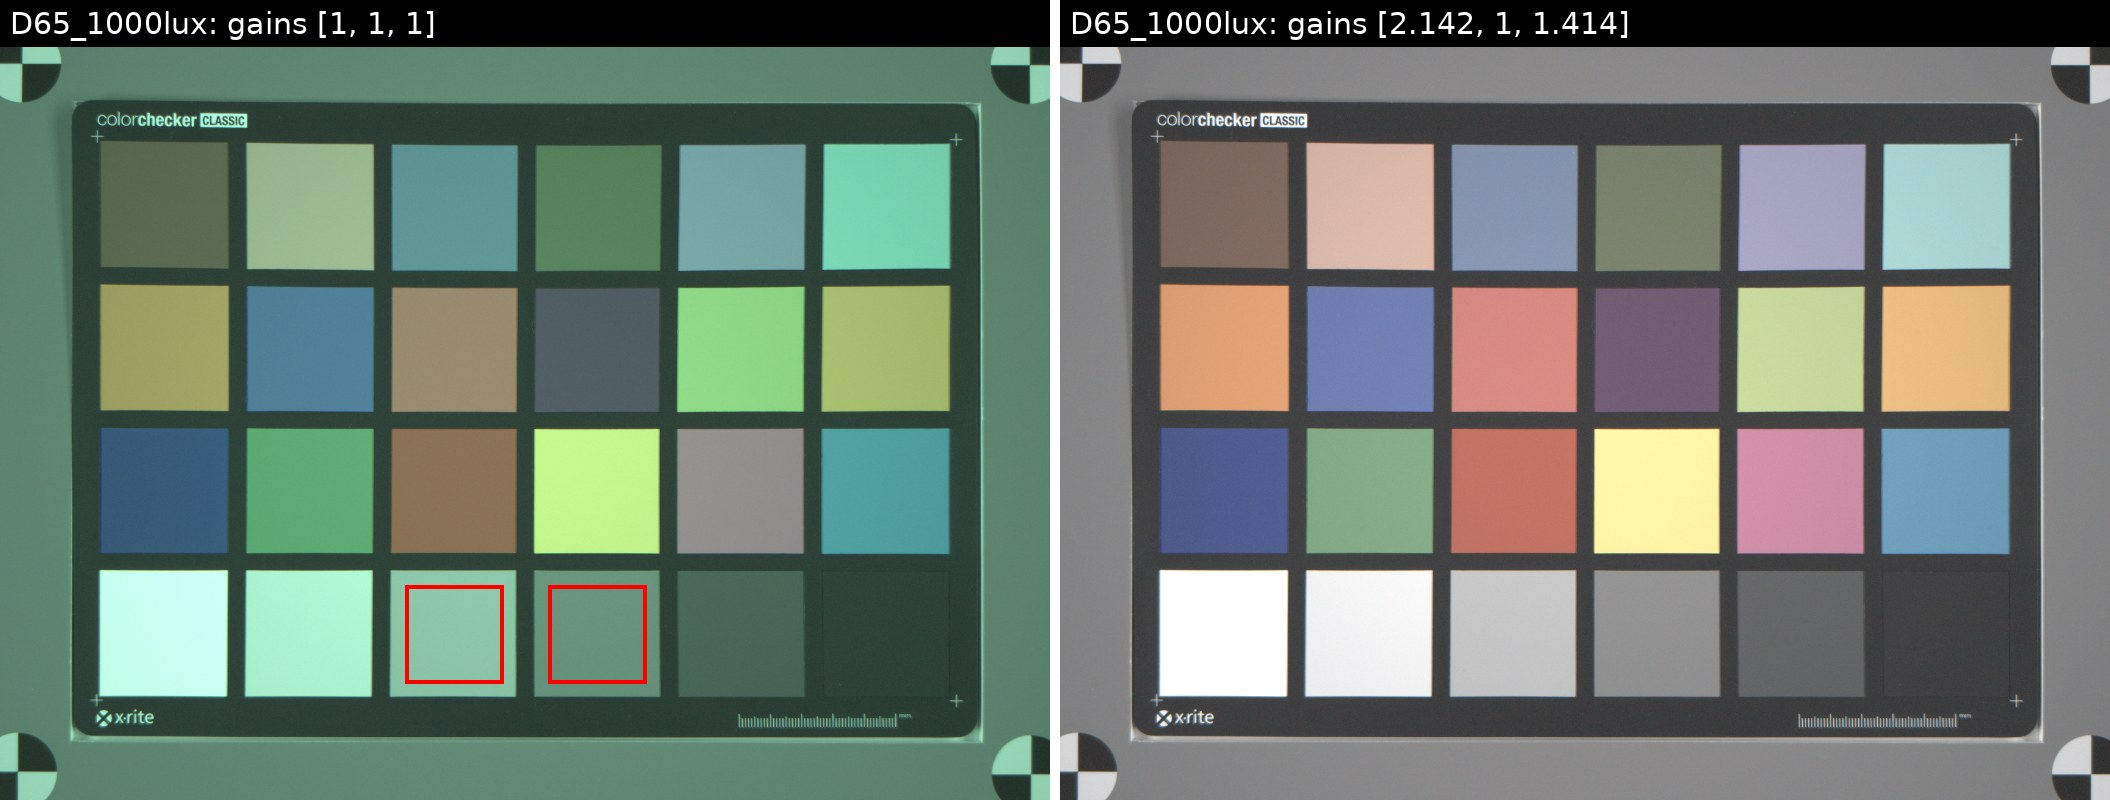
\includegraphics[width=0.8\linewidth]{CC_D65_1000lux_wb.jpg}\\[4pt]
  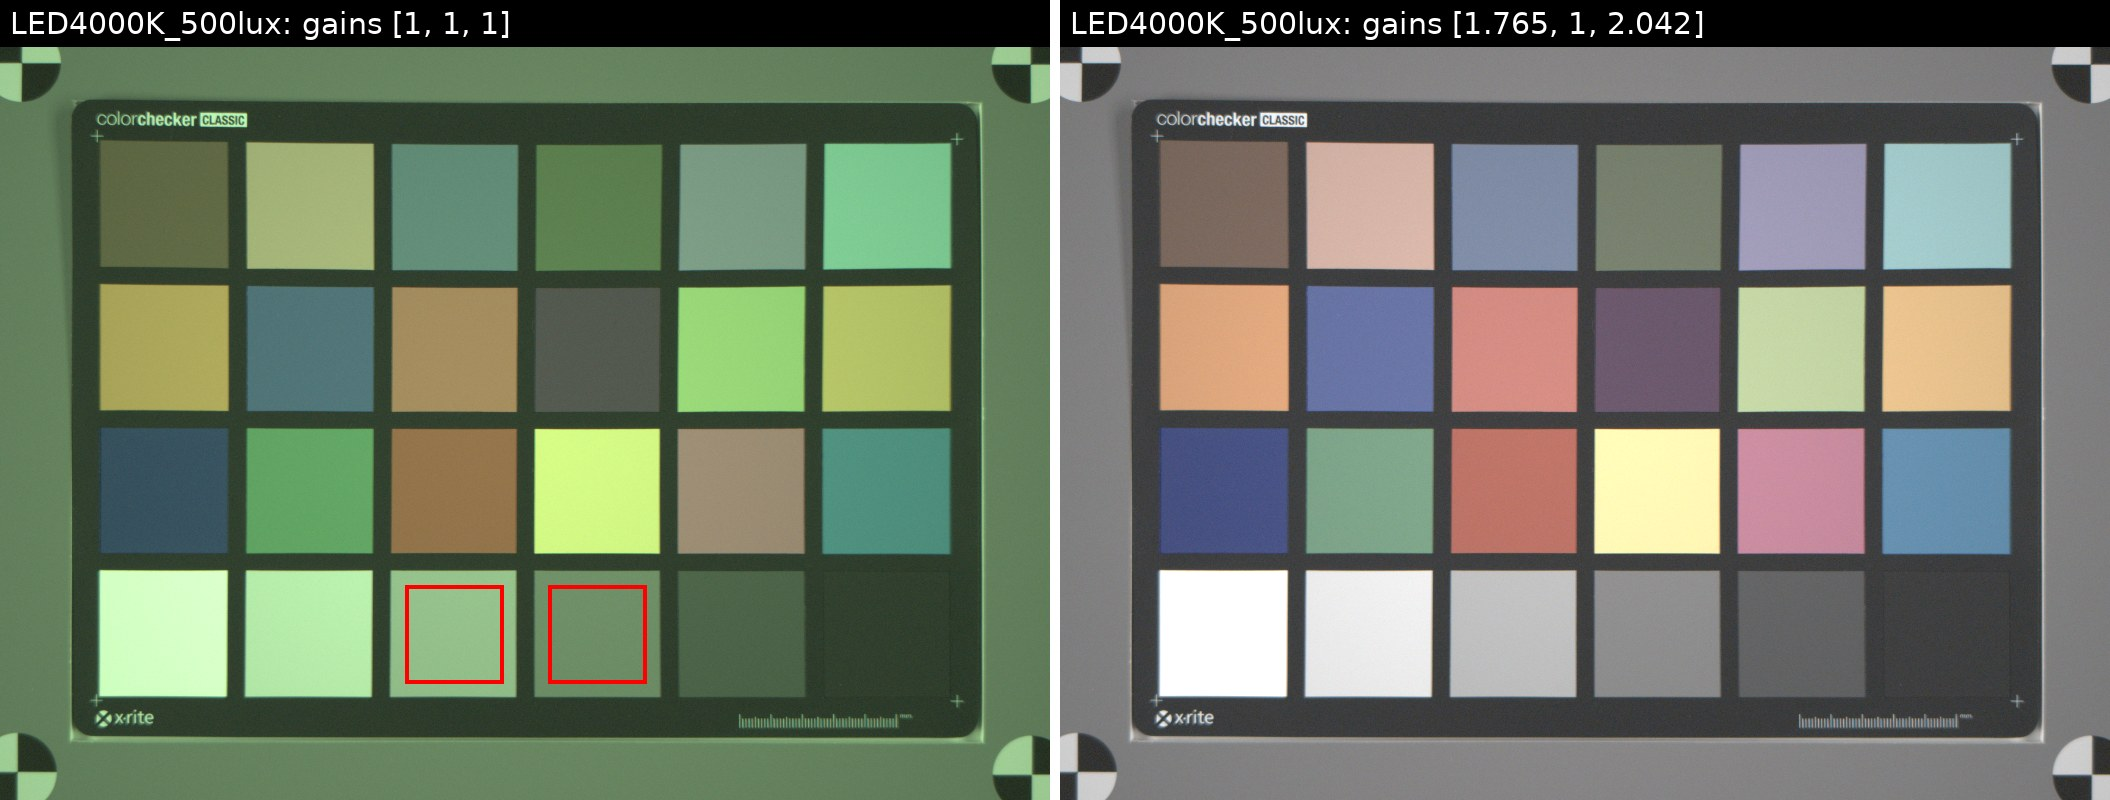
\includegraphics[width=0.8\linewidth]{CC_LED4000K_500lux_wb.jpg}\\[4pt]
  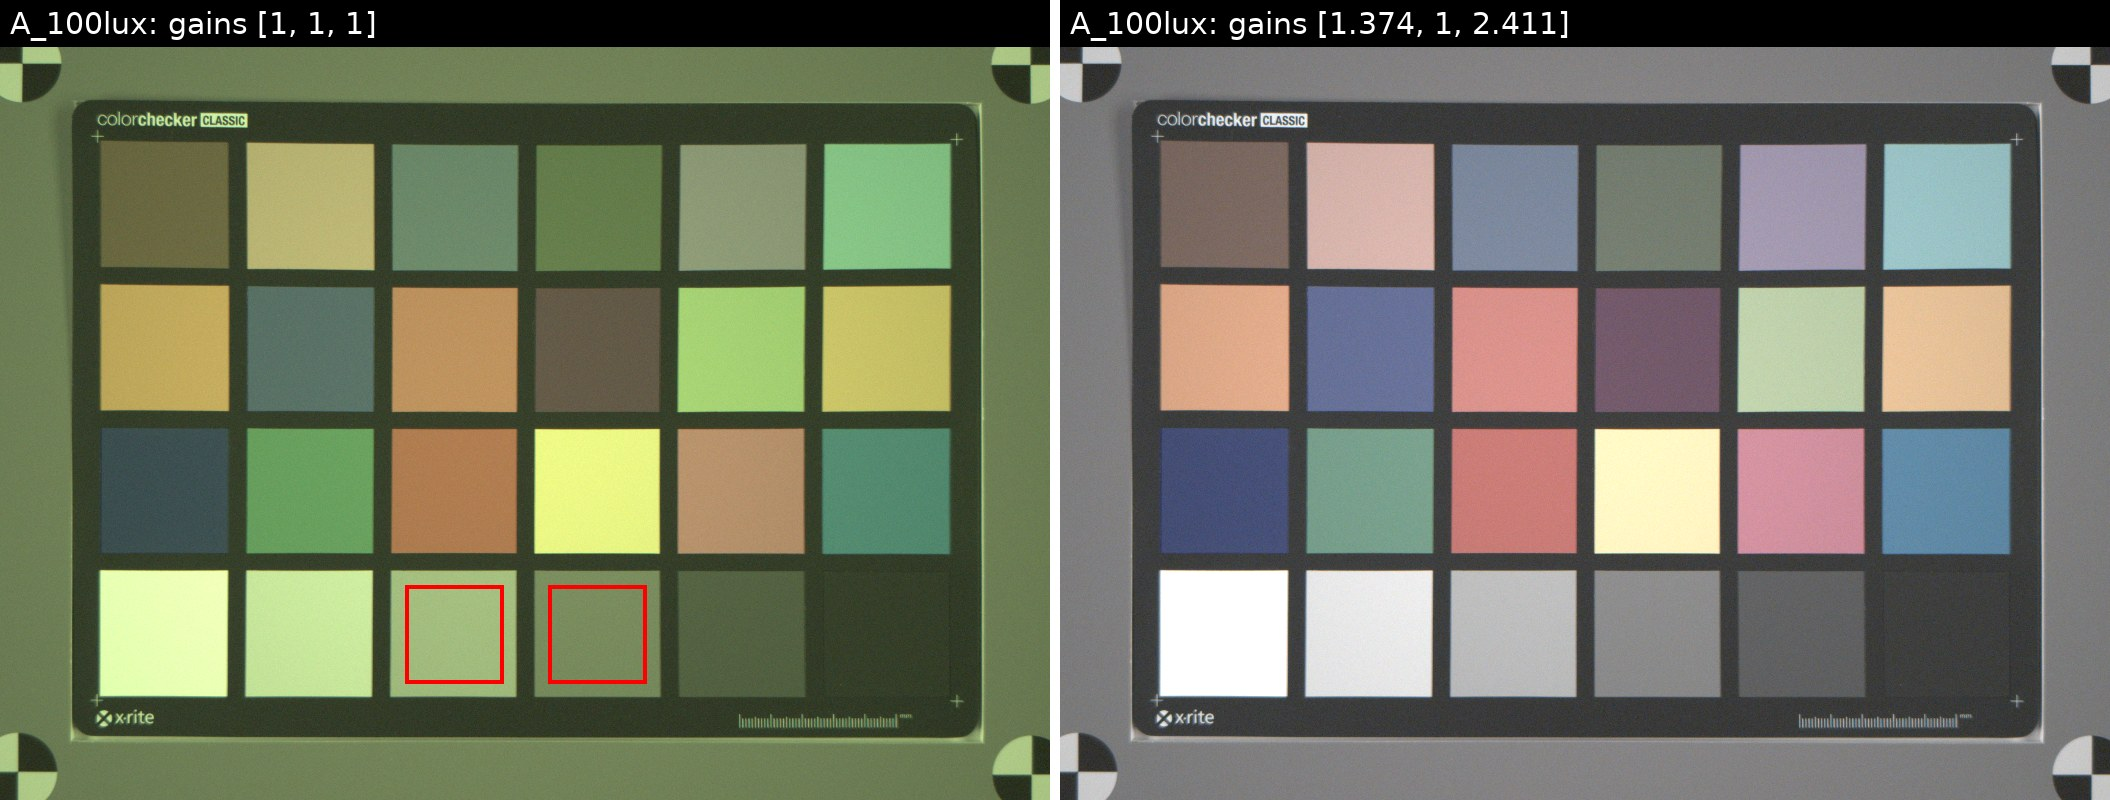
\includegraphics[width=0.8\linewidth]{CC_A_100lux_wb.jpg}
  \caption{ColorChecker under D65 (top), LED 4000K (middle) and CIE A (bottom).
           Left: gains $[1,1,1]$ with patches 21 and 22 marked.
           Right: calculated gains.}
  \label{fig:cc}
\end{figure}

The gains follow the spectra of the illuminants. D65 contains a lot of blue, so
the blue gain is the smallest and the red gain the largest. CIE A (2856\,K
tungsten) has little blue energy, so the blue gain is the largest (2.41) and
the red gain the smallest. LED 4000K lies in between. Both gains are above 1
for every illuminant because the green channel is the most sensitive one (its
spectral response is the widest and sits in the middle of the visible range).

\subsection{Why patches 21 and 22 instead of white or black?}

\begin{itemize}
  \item \textbf{No clipping.} The white patch (19) reflects about 90\,\% of the
        light, so at least one channel can reach or approach saturation (1023).
        A clipped channel underestimates its mean and gives a wrong ratio.
        Patches 21 and 22 (about 36\,\% and 20\,\% reflectance) stay well inside
        the linear range of the sensor.
  \item \textbf{Good signal-to-noise ratio.} The black patch (24) gives values
        close to the black level, where read noise, dark current and any
        remaining black-level error dominate. Small absolute errors there turn
        into large errors in $G/R$ and $G/B$. The mid-grey patches have plenty
        of signal.
  \item \textbf{Spectrally flat.} Patches 21 and 22 are designed to be
        spectrally neutral, so the ratio between channels reflects only the
        illuminant and the sensor, not the patch.
  \item \textbf{Two patches} at different levels average out noise and small
        non-linearities and reflectance deviations of a single patch.
\end{itemize}

\subsection{Why should the patch start on an odd row and column?}

The raw image is a Bayer mosaic that repeats every $2 \times 2$ pixels (GBRG
for this sensor). MATLAB indexing starts at 1, so pixel (1,1) is G, (1,2) is B,
(2,1) is R and (2,2) is G. If the extracted region starts on an odd row and odd
column, it has the same $2 \times 2$ phase as the full image, and the
sub-sampling \texttt{(1:2:end, 2:2:end)} etc.\ picks out the correct colour
channel. If the region started on an even row or column, the pattern would be
shifted (for example to RGGB or BGGR) and R, G and B values would be mixed up,
giving wrong gains.

%--------------------------------------------------------------------
\section{Part 2: Gain comparison and analysis}

Each test image was processed with the MATLAB ISP simulator using the
calculated gains, the simulator's default gains (\texttt{calculateWhiteBalance}
returning \texttt{[]}) and gains $[1, 1, 1]$.

\begin{figure}[H]
  \centering
  \begin{subfigure}{0.32\linewidth}
    \simimg{test_D65_calculated.png}{Calculated $[2.142, 1, 1.414]$}
  \end{subfigure}\hfill
  \begin{subfigure}{0.32\linewidth}
    \simimg{test_D65_default.png}{Default gains}
  \end{subfigure}\hfill
  \begin{subfigure}{0.32\linewidth}
    \simimg{test_D65_ones.png}{Gains $[1, 1, 1]$}
  \end{subfigure}
  \caption{\texttt{test\_D65\_1000lux.dng}}
\end{figure}

\begin{figure}[H]
  \centering
  \begin{subfigure}{0.32\linewidth}
    \simimg{test_LED4000K_calculated.png}{Calculated $[1.765, 1, 2.042]$}
  \end{subfigure}\hfill
  \begin{subfigure}{0.32\linewidth}
    \simimg{test_LED4000K_default.png}{Default gains}
  \end{subfigure}\hfill
  \begin{subfigure}{0.32\linewidth}
    \simimg{test_LED4000K_ones.png}{Gains $[1, 1, 1]$}
  \end{subfigure}
  \caption{\texttt{test\_LED4000K\_500lux.dng}}
\end{figure}

\begin{figure}[H]
  \centering
  \begin{subfigure}{0.32\linewidth}
    \simimg{test_A_calculated.png}{Calculated $[1.374, 1, 2.411]$}
  \end{subfigure}\hfill
  \begin{subfigure}{0.32\linewidth}
    \simimg{test_A_default.png}{Default gains}
  \end{subfigure}\hfill
  \begin{subfigure}{0.32\linewidth}
    \simimg{test_A_ones.png}{Gains $[1, 1, 1]$}
  \end{subfigure}
  \caption{\texttt{test\_A\_100lux.dng}}
\end{figure}

\subsection{What does it mean when the simulator uses gains $[1, 1, 1]$?}

It means that no white balancing is done: every channel is multiplied by one
and passed on unchanged. The image therefore keeps both the colour of the
illuminant and the unequal channel sensitivities of the sensor. Because the
green channel is the most sensitive, all images get a strong green cast. Under
CIE A it is yellow-green (little blue), under D65 green-cyan (little red), as
can be seen in the left-hand images of Figure~\ref{fig:cc}. Grey objects are no
longer grey, and the later colour correction matrix, which assumes
white-balanced input, cannot fix the colours properly.

\subsection{Calculated gains vs.\ default gains}

% TODO: replace this paragraph with what you see in the simulator outputs.
\textcolor{red}{[Describe the differences you observe in the images above.]}

The differences between the two results are caused by:
\begin{itemize}
  \item the default gains being fixed values that are not measured for the
        actual illuminant of the scene. If they are tuned for one illuminant
        (often D65), the D65 result looks very similar to the one with
        calculated gains, while A and LED 4000K show a remaining colour cast;
  \item the real light sources differing from the ideal CIE spectra (the
        measured spectra in the dataset do not exactly
        match the target spectra);
  \item noise, small lens-shading residuals and the choice of patches in the
        calculated gains.
\end{itemize}

Our calculated gains are within about 4\,\% of the as-shot white balance stored
in the DNG files by the phone (A: $[1.364, 1, 2.393]$,
D65: $[2.056, 1, 1.418]$, LED: $[1.744, 1, 2.044]$), which supports that the
method and the patch selection are correct.

%--------------------------------------------------------------------
\section{Conclusion}

A chart-based white balance using ColorChecker grey patches 21 and 22 gives
stable gains for all three illuminants. The gains match the illuminant spectra
and the phone's own white balance, and they make the grey patches neutral.
Without white balancing ($[1, 1, 1]$) the images show a strong colour cast,
which shows why the block is needed before demosaicing and colour correction.

%--------------------------------------------------------------------
\clearpage
\appendix
\section{\texttt{calculateWhiteBalance.m}}
\label{app:code}

\begin{lstlisting}
function wb_gains = calculateWhiteBalance(input_image)
    img = double(input_image);
    [H, W, ~] = size(img);

    % Patch boxes [rowStart rowEnd colStart colEnd], ~80 % of each patch,
    % measured on the 3072 x 4080 ColorChecker captures.
    refSize  = [3072 4080];
    box21    = [1871 2066 1811 2006];   % gray patch 21
    box22    = [1871 2066 2097 2292];   % gray patch 22
    boxWhite = [1871 2066 1229 1424];   % white patch 19 (orientation check)

    % Scale the boxes if the image size differs from the reference.
    scale = [H H W W] ./ [refSize(1) refSize(1) refSize(2) refSize(2)];
    box21    = makeOddStart(round(box21    .* scale));
    box22    = makeOddStart(round(box22    .* scale));
    boxWhite = makeOddStart(round(boxWhite .* scale));

    % Rotate back if the capture is upside down (white patch check).
    rotWhite = [H+1-boxWhite(2) H+1-boxWhite(1) W+1-boxWhite(4) W+1-boxWhite(3)];
    if meanOf(img, rotWhite) > meanOf(img, boxWhite)
        img = rot90(img, 2);
    end

    % Extract the patches, average per channel, compute gains.
    gains21 = patchGains(extractPatch(img, box21));
    gains22 = patchGains(extractPatch(img, box22));

    % Average the gains of the two patches.
    wb_gains = (gains21 + gains22) / 2;
end

function patch = extractPatch(img, box)
    patch = img(box(1):box(2), box(3):box(4), :);
end

function gains = patchGains(patch)
    if size(patch, 3) == 3
        R_avg = mean(patch(:, :, 1), 'all');
        G_avg = mean(patch(:, :, 2), 'all');
        B_avg = mean(patch(:, :, 3), 'all');
    else
        % GBRG: top-left pixel of the patch is G.
        G1 = patch(1:2:end, 1:2:end);
        B  = patch(1:2:end, 2:2:end);
        R  = patch(2:2:end, 1:2:end);
        G2 = patch(2:2:end, 2:2:end);
        R_avg = mean(R(:));
        G_avg = mean([G1(:); G2(:)]);
        B_avg = mean(B(:));
    end
    gains = [G_avg / R_avg, 1, G_avg / B_avg];
end

function m = meanOf(img, box)
    p = extractPatch(img, box);
    m = mean(p(:));
end

function box = makeOddStart(box)
    box([1 3]) = box([1 3]) - (mod(box([1 3]), 2) == 0);
end
\end{lstlisting}

\end{document}
